To evaluate the combination of these methods in the context of GVGP, the competition parameters of the 2018 GVGAI Learning track were used.
More information about these rules can be found in the 2019 GVGAI survey\cite{GVGAI19}.
As the validation levels for the 2018 track haven't been released at the time of writing, 3 games from the set were chosen to run be the games to train and test on.
\par
The chosen games were Aliens, Missile Command and Boulderdash.
These games were chosen based upon the results of the initial paper for the GVGAI gym framework by Torrado et al.\cite{GVGAIGym}.
While Torrado et al. used the same network and hyperparameters during training, they trained each game separately and only trained upon a single level.
This gives a good starting point to show what games and hyperparameters could work well for general video game playing.
\par
For each of the games levels 0 and 1 were used for training and levels 2,3 and 4 were used for validation.
The same settings were used as in section~\ref{ssec:experimentalMethod} while trained for 100 million frames of gameplay with the same combined parameters described in section~\ref{sssec:allCombined}, these resulting network is labelled model 1.
A further 2 models were trained based off the VGG16 architecture first described by Simonyan and Zisserman as an example of how current deep CNNs work~\cite{VGG16}.
The both used a screen warping size of 128x128 and both trained for less time before plateauing, at 17 million and 10 million time-steps, for model 2 and 3 respectively.
Model 3 uses the same architecture described by Simonyan and Zisserman~\cite{VGG16} only changing the output layer to the desired size.
Model 2 used the same feature extraction as VGG16 but has fewer nodes in the hidden MLP layers at 128 and 64. 

\subsection{Qualitative Results}
In this section the performance of the final trained agent is evaluated qualitatively by running the trained agent in both the training and validation levels.
\subsubsection{Aliens}
Performance on Aliens was quite interesting, while the agent performed well it struggled to shoot the aliens with the precision that you might expect from perfect play.
This could be due to how the agent has no perception of time and therefore the speed and direction the aliens are moving at.
\par
Its ability to shoot down aliens degrades the further the aliens appear down the screen, which could be due to it having little experience in those situations.
While all levels currently available have the aliens spawn in the upper left hand corner of the screen, aliens spawning elsewhere could be a problem to this agent.
\par
As the barriers provide points for destroying them the agent employs a rather reckless strategy of getting rid of its defensive to maximise points while simply dodging all incoming missiles.
\subsubsection{Missile Command}
\label{sssec:qualMC}
During the training levels of missile command there are only red missiles that the agent has to stop where as in the validation levels 2 and 3 there are blue missiles too.
In these levels the agents just ignore the blue missiles as it has never seen these before, resulting in some negative points and loses.
Level 4 is relatively similar to level 1 which explains why the agents perform well on it again.
\subsubsection{Boulderdash}
All agents struggled to win boulderdash due to win condition not having a reward associated with it.
It appeared that the agents significantly over fit to the 2 training levels with the agents appearing to move in a set pattern.
This meant that in one of the validation levels the agent tried to continuously move upwards even though it was at the top of the screen, this repeated behaviour also signifies a disadvantage of a purely reactive agent and architecture as, due to the state of the game not visually changing, the agent kept repeating the same useless action.
As a result the agents couldn't scored very poorly on the validation levels for boulderdash, showing it failed to generalise to new levels.
\subsubsection{All Games}
Unlike the planning agents there is no expectation that these agents could generalise to other games in the GVGAI framework as they haven't learnt to play them.
This puts these agents at a significant disadvantage currently compared to the vastly more general planning agents.
This effect can be seen as the competition organisers only expect the learning agents to perform in 3 games vs the 10 games that planning agents are evaluated in.

\subsection{Comparison with planning agents}
These three games were featured together in the GVGAI training set 1 for planning agents\cite{GVGAITrainingSet1} and was used during the CIG 2014 and 2015 GVGAI competitions.
As such planning agents created for these competitions (as well as other agents evaluated on the training set) can be downloaded and used to compare against.
Unfortunately at the time of writing there are no agents from the learning track that are available to download and run.
As the winner of the 2014 competition adrienctx was chosen as the agent to compare to, alongside a sample MCTS method and a random agent.

\subsection{Quantitative Results}
The graph in Figure~\ref{fig:aliensScore} compares the average score for all agents over 10 playthroughs of each level.
Note the dotted vertical line separates the training and test levels for the models.
\begin{figure}[ht]
  \centering
  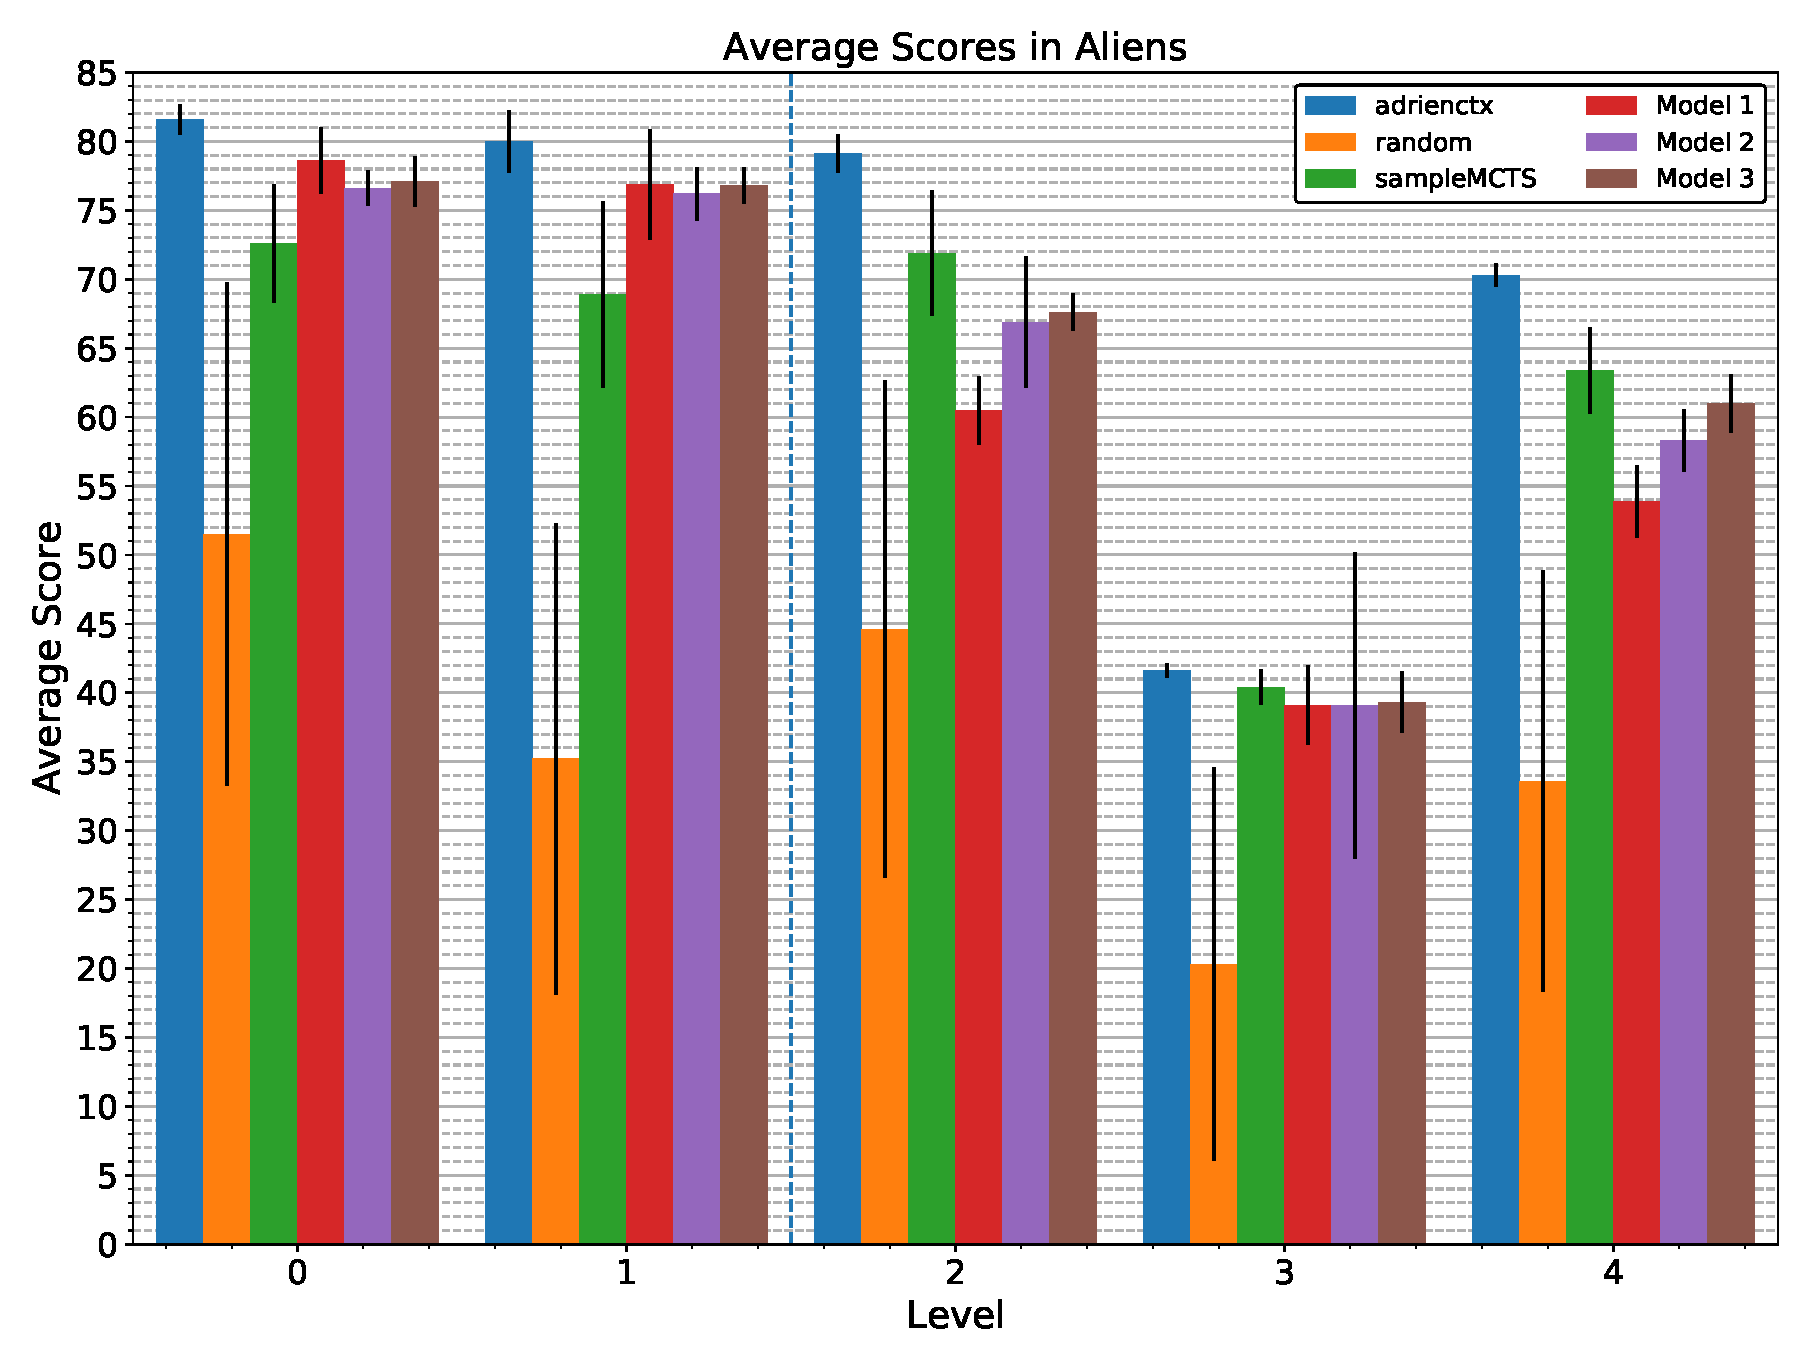
\includegraphics[width=0.7\linewidth]{graphs/FinalAliensScores.eps}
  \caption{Performance Comparisons with previous Agents}
  \label{fig:aliensScore}
\end{figure}
\par
While aliens was the closet game it is still clear that the planning agents have a slight advantage.
In Boulderdash acrienctx was the clear winner as it was the only agent to achieve wins on all 5 levels, but in Missile Command the model agents performed best, on levels 0,1 and 4 but couldn't win levels 2 and 3 due to the ignoring of blue missiles discusses in Section~\ref{sssec:qualMC}.
\par
An interesting point is that while running the model on a GTX 1080 GPU, the inference time of the model was approximately 5-8ms, significantly lower than the 40ms planning agents needed.
This would allow agents to play games at above 60fps vs the 24fps current planning agents play at, which is more comparable to the arcade games the GVGAI framework is based upon.
